\documentclass{jarticle}
\usepackage{robomech}
\usepackage[dvipdfmx]{graphicx}
\usepackage{amsfonts}
\usepackage{hyperref}

\begin{document}
\makeatletter
\title{価値反復を用いた移動ロボットによる屋外ナビゲーション}
{}
{Outdoor navigation with a mobile robot using value iteration}
{}

\author{
	\begin{tabular}{ll}
		○学\hspace{1zw}登内 リオン(千葉工大)& 正\hspace{1zw}林原 靖男\hspace{1zw} (千葉工大)\\
 		\hspace{1zw}正\hspace{1zw}上田 隆一(千葉工大)\\
		% ※協賛・後援団体の会員資格で発表される場合は「正・学」は不要です。
	\end{tabular}
	% &\\
	\vspace{1zh} \\
	\begin{tabular}{l}
			{\small Leon TONOUCHI, Chiba Institute of Technology, s20c1078un@s.chibakoudai.jp} \\
			{\small Ryuichi UEDA, Chiba Institute of Technology} \\
			{\small Yasuo HAYASHIBARA, Chiba Institute of Technology}             \\
	\end{tabular}
}
\makeatother

\abstract{ \small
We examine our software package for mobile robot navigation in the real world. 
This software uses value iteration for updating a decision making policy 
in the whole state space. Though the computational cost of this method
is too large for current computers, we expect that it will be standard
in future. In the experiments, we use this package with a laptop computer on
a mobile robot. Though the calculation time is still a problem,  
it works on the mobile robot for the first time. 
}

\date{} % 日付を出力しない
\keywords{robot navigation, brute-force value iteration}

\maketitle
\thispagestyle{empty}
\pagestyle{empty}

\small
\section{緒言}%===========================
%本文:明朝体・9pt(欧文Times New Roman, 9pt)、文字間隔は1行26文字程度、行間隔は4.2mm程度にして下さい。
価値反復は, ベルマン最適方程式を用いて, 
有限マルコフ決定過程における最適方策を正確に求めることができる手法である\cite{Shinjuku1}.
価値反復を移動ロボットの行動計画に適用すると,
環境中でロボットがとりうる全ての位置と向きに対して, 最適な行動を計算できる\cite{Shinjuku2}.
しかし, 経路計画によく用いられるA*\cite{Shinjuku3}などの探索手法よりも,
計算量が大きい。
だが, 計算機の性能向上でその問題が将来的に小さくなると,
探索手法よりも優れた解が得られ,
予期せぬ障害物に対しても, より効率のよい迂回経路を示すことができる.

上田らは, 現在の計算機でも,
限られた環境の広さであれば価値反復を利用できるのではないかと考え,
価値反復による経路計画のためのROSパッケージを実装した\cite{上田rsj2021}.
シミュレーション中では, 100$\mathrm{[m^2]}$超の環境において,
ハイエンドのノートパソコンで3秒程度の計算コストで
計画可能であることを示した.
しかし, パッケージ自体が実際の移動ロボットで試されたことはない.
実際の移動ロボットでは搭載できるノートパソコンの大きさや
利用できる電力に制限があり,
また, 計算能力に余力がないと, ロボットの動作が不安定になる可能性がある.


そこで本稿では, このパッケージを屋外移動ロボットで用い,
実機がこのパッケージで実際にナビゲーション可能かどうかと、
実環境での計算量を調査する。
2章で今回行った実験の環境や結果, 実験に用いるROSパッケージについて説明し, 
3章では結言を述べる.

%※ 講演番号、講演会名、ページ番号は記載しないようにして下さい。
\section{実装}%===========================

\subsection{価値反復ROSパッケージの実機への適用}

今回の実験では上田らが開発した価値反復ROSパッケージ
(\url{https://github.com/ryuichiueda/value_iteration}のコミット\texttt{22422bc}\dots)
\cite{上田rsj2021}をアールティ社のRaspberry Pi Catに適用した。
Raspberry Pi Catに、図\ref{fig:raspicat}のように
ノート型の計算機(ノートPC)を搭載し、
このノートPCのなかで、価値反復パッケージによる計算や、
自己位置推定などを実行する。
自己位置推定は、図中の2D LiDARで行う。
ノートPCは、CPUとしてIntel Core i7-11800H(8コア16スレッド)、
DRAMとしてDDR4-3200 64GBを持つノート型パソコン(ノートPC)
を搭載している。

\begin{figure}[htb]
  \centering
   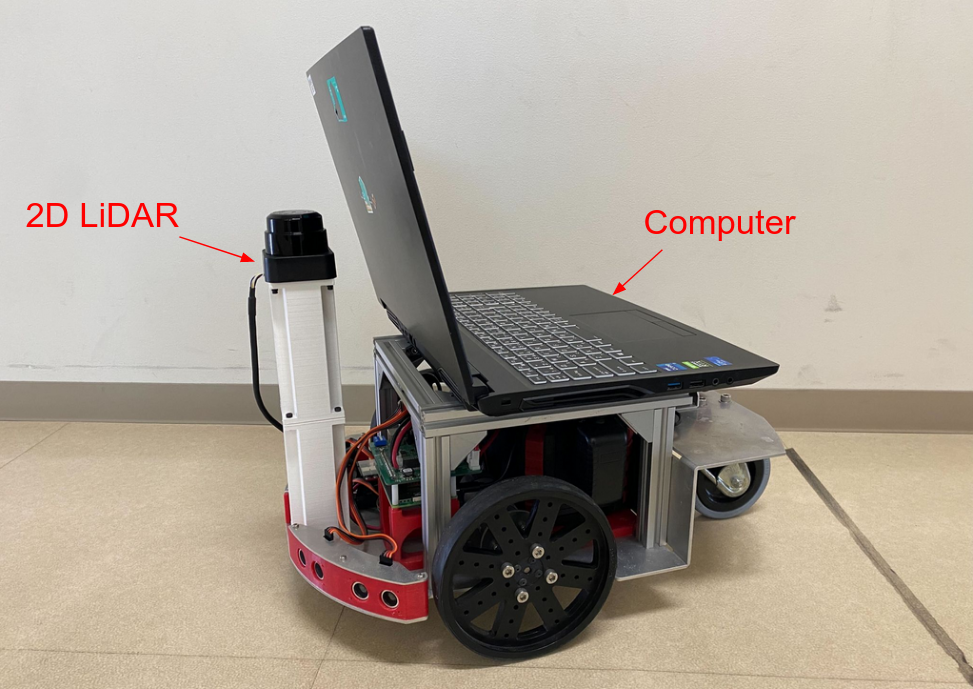
\includegraphics[height=53mm]{./figs/raspicat.png}
   \caption{Experimental setup}
	\label{fig:raspicat}
\end{figure}


@@@ここにパッケージの変更点を書く。ないならそう書く@@@

\subsection{環境と地図}

Raspberry Pi Catを走らせる環境は、
千葉工業大学津田沼キャンパスの敷地とした。
この環境を走らせるために、
図\ref{fig:tsudanuma}の地図を準備した。
形式は、ROSのナビゲーションスタックで用いられる
画像形式の占有格子地図であり、白色が
障害物のない画素、黒色が障害物のある画素、
灰色が不明な画素を表す。

\begin{figure}[htb]
  \centering
   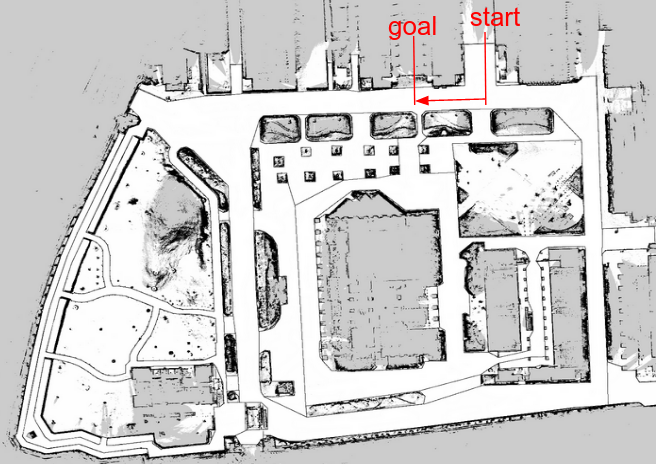
\includegraphics[height=53mm]{./figs/tsudanuma.png}
   \caption{the map for value iteration}
	\label{fig:tsudanuma}
\end{figure}

表\ref{table:map}に、この地図のパラメータ等を示す。
画素数は幅1962$\mathrm{[pixel]}$, 
高さ1333$\mathrm{[pixel]}$で、
1画素あたりの解像度は幅、高さとも150[mm]である。
計算量に大きく関係する白色の画素の面積は
$3.7\times 10^3$[m$^2$]と、\cite{上田rsj2021}
の実験の30倍を超える。

\begin{table}[hbt]
  \caption{configurations of the map}
	\label{table:map}
  \centering
	\begin{small}
  \begin{tabular}{l|r}
    \hline
    map size & 294.3 $\mathrm{[m]}\times 199.95\mathrm{[m]}$\\
    cell resolution &  0.15$\mathrm{[m]}\times 0.15\mathrm{[m]}$ \\
		number of cells & 2,615,346\\
    number of free cells & 165,076\\
		the area of the free cells & 3714.98$\mathrm{[m^2]}$\\
    \hline
  \end{tabular}
	\end{small}
\end{table}


\section{実験}%===========================

このROSパッケージ\cite{上田rsj2021}は, 2次元の離散化した占有格子地図を読み込み, 
ロボットの向きの1次元を加えた3次元の離散空間で経路計画を行っている.
地図(Fig. 1)のスタート地点から設定したゴール地点(15.6$\mathrm{[m]}$)まで10回走行させ, 価値反復の計算量を計測した.

自己位置推定には上田らが作成したROSのemclパッケージ(\href{https://github.com/ryuichiueda/emcl}{https://github.com/ryuichiueda/emcl})\cite{Shinjuku5}, 価値反復の際のコストの計算には占有格子地図を用いた.

Table 1には, 地図の大きさ, 格子の解像度, ロボットが移動できる地図のセルの数, 面積を記載する.
Table 2には, 価値反復の離散状態数と行動の数を記載する.
離散状態数は, 今回用いる地図のセルの数に, θ軸上の区分数(今回の実験では60)をかけたものである.
Table 3には, 6種類の行動と各行動の前進の速度と角速度を記載する.
この値は使用するロボットに合わせ, 適切だと考えられる値に調整したものである.




\begin{table}[hbtp]
	\caption{parameters for value iterations}
  \centering
  \begin{tabular}{l|r}
    \hline
    number of states & 156,920,760\\
    number of free states &  9,904,560\\
		number of actions & 6\\
    \hline
  \end{tabular}
	\caption{type of actions}
	\centering
	\begin{tabular}{l|cc}
 		\hline
		& forward & angular \\
 		type & versity[m/s] & versity[deg/s] \\
 		\hline \hline
 		forward & 0.3 & 0.0 \\
 		backward & -0.2 & 0.0 \\
 		right & 0.0 & -20.0 \\
 		left & 0.0 & 20.0 \\
 		right forward & 0.2 & -20.0 \\
 		left forward & 0.2 & 20.0 \\
	 \hline
	\end{tabular}
\end{table}

\subsection{並列処理}
価値反復のノード(vi\_node)は, 他のノードからゴールを指定されると即座に価値反復を開始する.
開始すると, 自己位置推定のノードから出力されるロボットの推定姿勢のトピックを受けて, 
その時点で得られる方策に基づいて行動(Table 3)を選択し, 選んだ行動に対応するロボットの速度を出力する.
価値反復のノードにはLinuxのPOSIXスレッドによる並列処理が導入されている. 
並列化されているのは, 状態遷移確率を求める処理と価値反復を行う処理である.

価値反復に用いるスレッドは設定で変更できるように実装されている. 
価値反復はロボットが動作しているときに実行されるため, 
演算に使用するスレッド数を多くしてしまうと, センサ処理の遅延などの悪影響が生じてしまう. 
しかし, スレッド数の増加によるナビゲーションにかかる時間の短縮と, 
物理コア数以上のスレッド数を用いた場合, 短縮の効果が頭打ちであるという結果が上田らの研究\cite{上田rsj2021}で示されている. 
よって本研究では, 使用する計算機の物理コア数が8コアであるため, スレッド数は8に固定して実験を行う.
\subsection{計算量の評価}
評価する方法としては, 上田らの研究\cite{上田rsj2021}と同様の方法を用いる. 
Fig. 1の「start」と書かれた地点から「goal」と書かれた地点まで, 
次の2通りの方法で, それぞれ10回ずつロボットを走行させ, かかった時間を測定する.

\begin{itemize}
	\item A: 価値反復中からロボットを動作させて計測
	\item B: 価値反復が終了したあとにロボットを動作させて計測
\end{itemize}

Aの場合, ロボットは価値反復の計算が完了する前に走行し始めるので, 開始時は最適ではない方策を用いる.
Bの場合, ロボットは価値反復の計算が完了してから走行し始める. 
この2通りの方法の時間の差(B-A)を実質的な計算時間とする.
\subsection{実験結果}
ロボットは価値反復の計算終了前に行動を開始するため, 次のAとBの実験の時間の差から実質的な計算時間を評価する. 
Table 4 に A と B のそれぞれの場合の実験結果を示す. 
A と B の計測の内容は以下のとおりである.

\begin{table}[hbtp]
	\caption{computational complexity}
	\centering
	 \begin{tabular}{l|cc}
		\hline
		 & average & standard \\
		 & of total time[s] & deviation[s] \\
		\hline \hline
		A & 123.3 & 6.2 \\
		B & 207.8 & 2.2 \\
		\hline
	 \end{tabular}
 \end{table}

Table 4には, Aの実験とBの実験それぞれでの計測した時間の平均と標準偏差を記載した. 
Aの実験の平均時間とBの実験の平均時間の差より, 今回の実験条件では実質的な価値反復の計算時間は84.6$\mathrm{[s]}$であった.

今回の実験では価値反復に用いる地図と自己位置推定に用いる地図の大きさを同じにしていた. 
そのため自己位置推定に悪影響を及ぼさない大きさの地図を使って計算量の評価を行っていた. 
しかし, 現在の地図の解像度だと価値反復の計算に時間がかかり過ぎてしまう. 
そのため, 価値反復に用いる地図と自己位置推定に用いる地図を別々にすることで, 価値反復に用いる地図を今以上に小さくすることができる. 
地図を小さくすることで, 離散状態数が減少し価値反復の計算にかかる時間が短くなると考えられる. 
\section{結言}%===========================
本稿では, 価値反復を用いた実時間経路計画アルゴリズムを屋外移動ロボットで用い, 屋外の実環境を走行させることで計算量を評価した. 
結果としては, 3714.98$\mathrm{[m^2]}$のフリースペースがある環境において, 
地図の解像度を0.15$\mathrm{[m/pixel]}$, 計算機としてIntel Core i7-11800Hを搭載したものを用いると, 
15.6$\mathrm{m}$走行し, 84.6$\mathrm{[s]}$も計算に時間がかかってしまうという結果が得られた. 
結果から, 屋外などの広い環境を想定した場合, 今回の実験の条件では価値反復の計算に時間がかかり過ぎてしまうため, 
屋外での走行を想定した移動ロボットへの適用は適切ではないと言える.

しかし, 価値反復に使用する地図の解像度をできる限り下げることで, 
離散状態数が小さくなるので, 価値反復の計算に用いる時間を短くすることができると考えられる.

今後は, 価値反復に用いる地図の解像度をどこまで下げることで, 
屋外を想定した移動ロボットへの適用が可能になるのかということを調査する. 

\footnotesize
\begin{thebibliography}{99}

	\bibitem{Shinjuku1}
	Bellman, R., {\it Dynamic Programming}, Princeton Uni-versity Press, Princeton, NJ, 1957.

	\bibitem{Shinjuku2}
	上田隆一,池邉龍宏,林原靖男,``移動ロボットのナビゲーションのためのbrute-forceな価値反復を用いた大域計画・局所計画アルゴリズム'', 
	第27回ロボティクスシンポジア講演論文集, 2022.
	
	\bibitem{Shinjuku3}
	Hart, P. E., Nilsson, N. J. and Raphael, B. ``A Formal
	Basis for the Heuristic Determination of Minimal Cost
	Paths,'' {\it IEEE Transactions on Systems Science and Cybernetics}, Vol. 4, No. 2, pp. 100-107, 1968.
	
	\bibitem{上田rsj2021}
	上田隆一,池邉龍宏,林原靖男,``brute-forceな価値反復を用いた実時間経路計画ROSパッケージ'', 
	第39回日本ロボット学会学術講演会予稿集, 2021.

	\bibitem{Shinjuku5}
	Ueda, R., {\it et al}., ``Real-Time Decision Making with State-Value Function under Uncertainty of State Estimation,''
	 in {\it Proc. of} ICRA, 2005.

	\bibitem{Shinjuku6}
	上田隆一,池邉龍宏,林原靖男,``価値反復による準静的な障害物を考慮した実時間経路'', 
	第40回日本ロボット学会学術講演会予稿集, 2022.

	\bibitem{Shinjuku2}
	上田隆一,登内リオン, 池邉龍宏,林原靖男,``移動ロボットのための自己位置の不確かさを考慮したセンシングできない固定障害物の回避方法'', 
	第28回ロボティクスシンポジア講演論文集, 2023.

\end{thebibliography}

\normalsize
\end{document}
